\chapter{Weak Fields, Gravitational Waves, and the Action Principle}

The exact equations of general relativity are nonlinear, and their component
form can become formidable before one has solved a single physical problem.
For the last lecture of the course, it is better to separate principle from
bookkeeping. We will ask what Einstein's equations become when the
gravitational field is weak, identify the waves contained in that
approximation, and then finish by seeing how the full field equations fit
inside a remarkably compact action principle.

Three questions organize the discussion. What does a weak gravitational
field mean? Why is the weak theory linear although the exact theory is not?
And what physical effects distinguish a gravitational wave from a mere
wiggle of coordinates?

\section{A Small Disturbance of an Equilibrium Geometry}

Weakness is an approximation scheme. If a dimensionless disturbance is of
size \(\epsilon\ll1\), its square is of size \(\epsilon^2\), and a
first-order calculation consistently discards the latter. The familiar
example is a mechanical system making small oscillations about equilibrium.
Its exact equations may be nonlinear, but sufficiently small oscillations
obey linear equations.

For gravity, the equilibrium background will be empty flat spacetime. Begin
with Einstein's vacuum equation,
\begin{equation}
 R_{\mu\nu}-\frac12 g_{\mu\nu}R=0.
 \label{eq:vacuum-einstein}
\end{equation}
Taking its trace in four dimensions gives
\begin{equation}
 g^{\mu\nu}
 \left(R_{\mu\nu}-\frac12 g_{\mu\nu}R\right)
 =R-2R=-R=0,
\end{equation}
so the vacuum equation is equivalently
\begin{equation}
 R_{\mu\nu}=0.
 \label{eq:ricci-flat}
\end{equation}

\begin{figure}[htbp]
\centering

\includegraphics[width=0.68\textwidth]{lecture_10_figure_02.png}
\caption{The vacuum equation \(R_{\mu\nu}=0\), isolated at the beginning of
the weak-field argument.}
\lectureframe{00:03:11}
\end{figure}

Here equilibrium means a source-free solution with no time dependence. Flat
spacetime is the simplest such solution. One qualification is essential:
flatness does not mean that the components of the metric equal a particular
matrix in every coordinate system. It means that inertial coordinates can
be chosen in which
\begin{equation}
 g_{\mu\nu}=\eta_{\mu\nu}.
\end{equation}
This distinction between a geometry and the coordinates used to describe it
will soon become the central subtlety.

Now imagine a violent source such as a compact binary. Its near field may be
strong, but far from the source the disturbance spreads out and becomes
small. In a suitable coordinate system the metric can then be written
\begin{equation}
 g_{\mu\nu}(x)=\eta_{\mu\nu}+h_{\mu\nu}(x),
 \qquad |h_{\mu\nu}|\ll1.
 \label{eq:weak-split}
\end{equation}
The perturbation \(h_{\mu\nu}\) is allowed to depend on all four spacetime
coordinates. Weakness means that powers beyond the first will be neglected.

\section{What Survives at First Order}

The complete Ricci tensor is too long to be useful at this stage. Its
structure is enough. Christoffel symbols contain an inverse metric and one
derivative of the metric, while curvature contains a derivative of a
Christoffel symbol and a product of two Christoffel symbols:
\begin{equation}
 \Gamma\sim\frac12 g^{-1}\partial g,
 \qquad
 R\sim\partial\Gamma+\Gamma\Gamma.
 \label{eq:curvature-skeleton}
\end{equation}

\begin{figure}[htbp]
\centering

\includegraphics[width=0.84\textwidth]{lecture_10_figure_03.png}
\caption{The weak-field split and the schematic construction
\(R\sim\partial\Gamma+\Gamma\Gamma\). The notation exposes the orders in
\(h\) without expanding every index.}
\lectureframe{00:10:17}
\end{figure}

The inverse metric follows from
\(g^{\mu\alpha}g_{\alpha\nu}=\delta^\mu{}_\nu\). To first order,
\begin{equation}
 g^{\mu\nu}=\eta^{\mu\nu}-h^{\mu\nu}+O(h^2),
 \label{eq:inverse-weak}
\end{equation}
where indices on \(h\) are raised with the background metric. In inertial
coordinates the background is constant,
\begin{equation}
 \partial_\alpha\eta_{\mu\nu}=0,
\end{equation}
and therefore
\begin{equation}
 \partial_\alpha g_{\mu\nu}
 =\partial_\alpha h_{\mu\nu}.
\end{equation}
Consequently,
\begin{equation}
 \Gamma=O(\partial h),
 \qquad
 R_{\mu\nu}
 =O(\partial\partial h)+O\bigl((\partial h)^2\bigr)
  +O(h\,\partial\partial h).
 \label{eq:ricci-orders}
\end{equation}

\begin{figure}[htbp]
\centering

\includegraphics[width=0.84\textwidth]{lecture_10_figure_04.png}
\caption{The board expansion of the inverse metric and the observation that
\(\partial\eta=0\). Only derivatives of \(h_{\mu\nu}\) remain at leading
order.}
\lectureframe{00:11:55}
\end{figure}

The last two terms in Equation~\eqref{eq:ricci-orders} are quadratic in the
disturbance and are omitted. The vacuum equations are therefore linear
equations involving second derivatives of \(h_{\mu\nu}\). This is the whole
meaning of linearization. It is not an assertion that Einstein's exact
theory is linear.

\begin{classroomqa}
\audiencequestion{The curvature tensor has four indices, while the Ricci
tensor has two. If two derivatives already carry indices and
\(h_{\mu\nu}\) carries two more, how does the index count work?}
\lecturerresponse{The Ricci tensor is obtained by contracting a pair of
indices in the curvature tensor. The metric used in that contraction leaves
two free indices, exactly the pair carried by \(R_{\mu\nu}\). The symbolic
form \(\partial\partial h\) suppresses those contractions; it is an order
count, not a complete indexed formula.
\lecturetimestamp{00:18:45--00:19:53}}
\end{classroomqa}

\begin{classroomqa}
\audiencequestion{Does contracting with the inverse metric introduce terms
such as \(h\,\partial^2h\), and if so, why may they be ignored?}
\lecturerresponse{It does. Replacing \(g^{-1}\) by
\(\eta^{-1}-h+\cdots\) produces both the linear term
\(\eta^{-1}\partial^2h\) and corrections containing a second \(h\). The
latter are quadratic. The same rule discards
\(h\,\partial h\), \(h\,\partial^2h\), and
\((\partial h)^2\). Keeping only one power of the perturbation is precisely
the approximation being made.
\lecturetimestamp{00:19:55--00:21:14}}
\end{classroomqa}

\section{Why the Equations Look Like Waves}

Second-derivative field equations naturally suggest wave propagation. For a
scalar function moving along the \(z\)-axis, the prototype is
\begin{equation}
 \left(\partial_t^2-\partial_z^2\right)\phi=0,
\end{equation}
whose solutions include arbitrary right- and left-moving profiles,
\begin{equation}
 \phi(z,t)=f(z-t)+g(z+t).
\end{equation}
In three spatial dimensions the same equation is
\begin{equation}
 \left(\partial_t^2-\nabla^2\right)\phi=0.
\end{equation}
Its linearity permits superposition: the sum of two solutions is another
solution.

Gravity is not a scalar field. The perturbation has tensor components, and
the equation \(R_{\mu\nu}=0\) initially appears to supply many component
equations. They are not all independent; some are constraints and some
reflect coordinate freedom. The analogy is with Maxwell theory, where a
family of field equations eventually leaves only the physical transverse
waves.

After suitable coordinate conditions are imposed, the radiative components
obey an ordinary wave equation,
\begin{equation}
 \Box h_{\mu\nu}=0,
 \qquad
 \Box=\eta^{\alpha\beta}\partial_\alpha\partial_\beta.
 \label{eq:linear-wave}
\end{equation}
The precise signs inside \(\Box\) depend on the signature convention; its
content does not. Disturbances propagate on the light cone.

\section{Coordinate Wiggles Are Not Gravitational Waves}

Before accepting every solution of the linearized equations as a physical
wave, we must return to the coordinate caveat. Flat space can be described
with curved coordinate lines. Its metric components then differ from their
Cartesian values even though its curvature is still zero.

The blackboard itself supplies the example. Draw straight Cartesian
coordinates on its flat surface and write
\begin{equation}
 ds^2=\delta_{mn}\,dx'^m dx'^n.
\end{equation}
Now relabel the same points with slightly wiggly coordinates,
\begin{equation}
 x'^m=x^m+f^m(x).
 \label{eq:small-coordinate-change}
\end{equation}
The differentials become
\begin{equation}
 dx'^m=dx^m+\partial_n f^m\,dx^n.
\end{equation}
Substituting into the line element and retaining only first order in \(f\)
gives
\begin{align}
 ds^2
 &=
 \delta_{mn}dx^m dx^n
 +\left(\partial_m f_n+\partial_n f_m\right)dx^m dx^n
 +O(f^2).
\end{align}
Thus an apparent perturbation of the form
\begin{equation}
 h_{mn}=\partial_m f_n+\partial_n f_m
 \label{eq:pure-gauge}
\end{equation}
can describe no new geometry at all. It is flat space in wiggly coordinates.

\begin{figure}[htbp]
\centering

\includegraphics[width=0.84\textwidth]{lecture_10_figure_05.png}
\caption{The coordinate-wiggle calculation on the board. A small
re-coordinatization induces a small-looking \(h_{mn}\) even though the
blackboard remains flat.}
\lectureframe{00:27:54}
\end{figure}

Equation~\eqref{eq:pure-gauge} is the linearized form of coordinate, or
gauge, freedom. Additional conditions are needed to eliminate these phony
perturbations. The detailed gauge algebra is not developed here. Its role is
the important point: it removes changes of description while preserving
changes of curvature. Once the coordinate freedom and the constraint
equations have been accounted for, the physical content reduces to two
independent wave polarizations.

\begin{figure}[htbp]
\centering
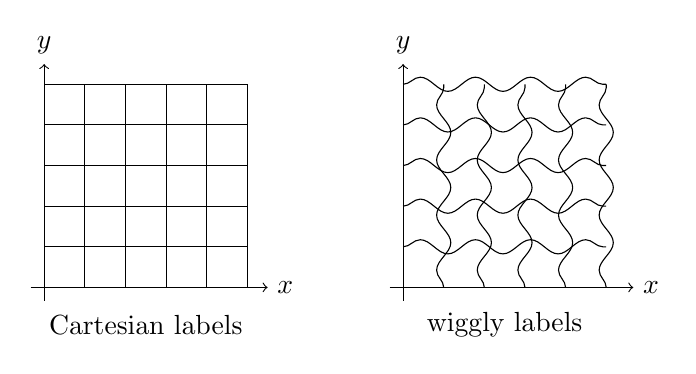
\begin{tikzpicture}[scale=0.86]
\begin{scope}
\draw[->] (-0.2,0) -- (3.3,0) node[right] {$x$};
\draw[->] (0,-0.2) -- (0,3.3) node[above] {$y$};
\foreach \u in {0.6,1.2,1.8,2.4,3.0}{
  \draw (\u,0) -- (\u,3.0);
  \draw (0,\u) -- (3.0,\u);
}
\node at (1.5,-0.55) {Cartesian labels};
\end{scope}
\begin{scope}[xshift=5.3cm]
\draw[->] (-0.2,0) -- (3.4,0) node[right] {$x$};
\draw[->] (0,-0.2) -- (0,3.3) node[above] {$y$};
\foreach \u in {0.6,1.2,1.8,2.4,3.0}{
  \draw[decorate,decoration={snake,amplitude=0.09cm,segment length=0.7cm}]
    (\u,0) -- (\u,3.0);
  \draw[decorate,decoration={snake,amplitude=0.09cm,segment length=0.7cm}]
    (0,\u) -- (3.0,\u);
}
\node at (1.5,-0.55) {wiggly labels};
\end{scope}
\end{tikzpicture}
\caption{The geometry stays flat while the coordinate grid changes. Metric
components alone cannot decide whether a perturbation is physical.}
\end{figure}

\section{A Wave Moving Along the z-Axis}

Choose a plane wave traveling in the positive \(z\)-direction. Its phase may
be written
\begin{equation}
 k(z-t),
\end{equation}
so a representative component has the form
\begin{equation}
 h_{\mu\nu}(z,t)
 =h_{\mu\nu}^{(0)}\sin k(z-t).
 \label{eq:plane-wave}
\end{equation}
Surfaces of constant phase satisfy \(z-t=\text{constant}\); the propagation
speed is therefore the speed of light.

In a transverse-traceless description, the components containing a time
index or a \(z\)-index vanish:
\begin{equation}
 h_{0\mu}=0,
 \qquad
 h_{z\mu}=0.
 \label{eq:tt-transverse}
\end{equation}
Only the \(x\)-\(y\) block remains. It is symmetric and traceless,
\begin{equation}
 h_{xy}=h_{yx},
 \qquad
 h_{xx}+h_{yy}=0.
 \label{eq:tt-trace}
\end{equation}

\begin{figure}[htbp]
\centering

\includegraphics[width=0.84\textwidth]{lecture_10_figure_06.png}
\caption{A wave traveling along \(z\), represented as a stack of transverse
planes. The surviving \(x\)-\(y\) amplitudes obey
\(h_{xx}+h_{yy}=0\).}
\lectureframe{00:43:36}
\end{figure}

There are consequently two independent patterns. They may be displayed as
\begin{equation}
 h^{\mathrm{TT}}_{ij}(z,t)
 =
 \begin{pmatrix}
 h_+ & h_\times\\
 h_\times & -h_+
 \end{pmatrix}
 \sin k(z-t),
 \qquad i,j\in\{x,y\}.
 \label{eq:polarization-matrix}
\end{equation}
The diagonal pattern is called the plus polarization. The off-diagonal
pattern is called the cross polarization. Rotating the transverse axes by
\(45^\circ\) turns one pattern into the other, and an arbitrary linearly
polarized wave is a superposition of the two. There are no further
independent polarizations in this theory.

\begin{figure}[htbp]
\centering
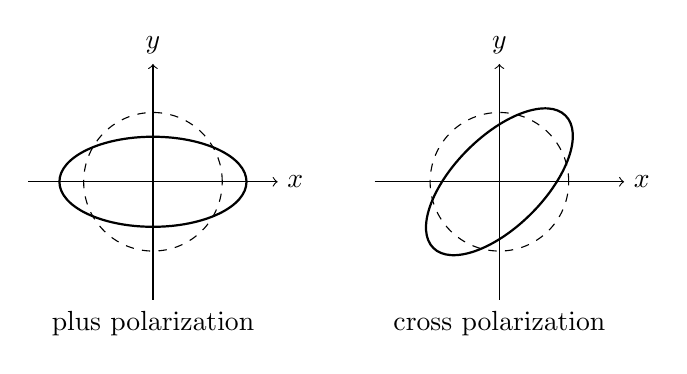
\begin{tikzpicture}[scale=0.88]
\begin{scope}
\draw[->] (-1.8,0) -- (1.8,0) node[right] {$x$};
\draw[->] (0,-1.7) -- (0,1.7) node[above] {$y$};
\draw[dashed] (0,0) circle (1.0);
\draw[thick] (0,0) ellipse (1.35 and 0.65);
\node at (0,-2.05) {plus polarization};
\end{scope}
\begin{scope}[xshift=5.0cm]
\draw[->] (-1.8,0) -- (1.8,0) node[right] {$x$};
\draw[->] (0,-1.7) -- (0,1.7) node[above] {$y$};
\draw[dashed] (0,0) circle (1.0);
\draw[thick,rotate=45] (0,0) ellipse (1.35 and 0.65);
\node at (0,-2.05) {cross polarization};
\end{scope}
\end{tikzpicture}
\caption{One half-cycle stretches one transverse direction while squeezing
the perpendicular direction. Half a cycle later the deformation reverses.}
\end{figure}

\section{From Metric Components to Physical Strain}

Fix \(z\) and \(t\) and inspect the transverse plane. For a pure plus wave,
\begin{equation}
 ds_\perp^2
 =(1+h_{xx})\,dx^2+(1-h_{xx})\,dy^2.
 \label{eq:transverse-distance}
\end{equation}
When \(h_{xx}>0\), a fixed coordinate interval in the \(x\)-direction has a
slightly larger proper length, while the corresponding \(y\)-interval has a
slightly smaller proper length. Half a period later \(h_{xx}\) changes sign,
and the roles reverse. A square is alternately stretched horizontally and
squeezed vertically, then squeezed horizontally and stretched vertically.
For the cross polarization, the same alternation occurs along axes rotated
by \(45^\circ\).

To first order, an arm initially of length \(L\) changes by
\begin{equation}
 \frac{\Delta L}{L}\simeq\frac12 h_{ij}n^i n^j,
 \label{eq:fractional-strain}
\end{equation}
where \(\mathbf n\) points along the arm. This formula translates the metric
perturbation into the dimensionless strain measured by a detector.

\begin{classroomqa}
\audiencequestion{A meter stick is held together electromagnetically and
does not simply change its rest length with the coordinates. Should the
picture instead use freely separated test masses?}
\lecturerresponse{The distinction is important. A real rod has elasticity,
so the tidal field drives stresses inside it; a steel rod and a wooden rod
will generally respond by different amounts. Freely suspended test masses
avoid that particular elastic response and reveal relative acceleration more
directly. In either case the passing wave is not merely relabeling points.
Its time-dependent curvature produces a physical effect.
\lecturetimestamp{00:47:23--00:48:48}}
\end{classroomqa}

The precise local statement is geodesic deviation. For nearby freely falling
particles separated by \(\xi^i\),
\begin{equation}
 \frac{d^2\xi^i}{dt^2}
 =-R^i{}_{0j0}\,\xi^j.
 \label{eq:geodesic-deviation}
\end{equation}
In the weak transverse-traceless wave,
\begin{equation}
 R_{0i0j}=-\frac12\ddot h^{\mathrm{TT}}_{ij},
 \label{eq:tidal-curvature}
\end{equation}
so the oscillating metric generates alternating tidal acceleration. This is
why a time-dependent wave cannot be dismissed as a static choice of rulers.
It has nonzero curvature.

\begin{classroomqa}
\audiencequestion{What can measure the squeeze and stretch if every ruler in
the region is affected?}
\lecturerresponse{A strain gauge can register the genuine stress induced in
a material body. Better still, one can monitor the changing separation of
freely suspended masses. A static, uniform rescaling could be absorbed into
the measuring apparatus, but the oscillating curvature drives a response
that can be recorded.
\lecturetimestamp{00:51:10--00:52:02}}
\end{classroomqa}

\section{Sources and Detectors}

Electromagnetic waves are generated by moving charges and currents.
Gravitational waves are generated by moving distributions of mass and
energy. Conservation of energy and momentum rules out gravitational
monopole and dipole radiation for an isolated system, so the leading
radiative moment is quadrupolar. A compact binary supplies exactly the
needed changing quadrupole: two dense bodies orbit one another and launch
waves into the far field.

Close to the binary, spacetime is strongly curved and the linear expansion
of Equation~\eqref{eq:weak-split} is unreliable. Far away, the outgoing wave
spreads over a larger area, its amplitude becomes small, and the linearized
description becomes accurate. For an observer on the \(z\)-axis from the
source, the measurable stretching lies in the transverse \(x\)-\(y\) plane.

\begin{classroomqa}
\audiencequestion{Is the ruler in the drawing an abstract coordinate ruler
or a physical meter stick, and how could a variable ruler measure the
effect?}
\lecturerresponse{It may be a physical object, but then its material
properties matter. Curvature supplies the tidal stress; steel and wood need
not deform identically under it. Comparing their responses is already a
measurement. A cleaner detector replaces the rods by separated test masses
and measures their differential motion.
\lecturetimestamp{00:54:00--00:55:19}}
\end{classroomqa}

A resonant detector is one strategy. If a mechanical system has a natural
frequency near that of the incoming wave, the wave drives it coherently and
amplifies the response. An interferometer uses another strategy: mirrors
serve as test masses, and laser interference compares the effective lengths
of perpendicular arms. A plus-polarized wave lengthens one arm while
shortening the other, which is exactly the differential signal an
interferometer is designed to detect.

\begin{classroomqa}
\audiencequestion{Would this be the basis of a gravitational-wave detector?}
\lecturerresponse{Yes. A stiff rod barely changes, whereas freely suspended
end masses can undergo relative acceleration. One can also exploit resonance
so that a weak periodic drive produces a larger response. The expected
astrophysical strain is extraordinarily small, of order \(10^{-21}\), so
detector design is the art of turning that tiny differential motion into a
measurable signal.
\lecturetimestamp{00:55:20--00:57:10}}
\end{classroomqa}

\begin{classroomqa}
\audiencequestion{Is LIGO an example of such a detector?}
\lecturerresponse{Yes. Its basic observables come from laser light reflected
between mirrors in perpendicular arms. A gravitational wave changes the
relative optical path lengths and therefore the interference pattern. At
the time of this lecture the instrument had not yet made a direct
detection; that historical situation later changed.\editorialnote{The first
direct observation, GW150914, was recorded in 2015 and announced in 2016.}
\lecturetimestamp{00:57:16--00:58:05}}
\end{classroomqa}

\begin{classroomqa}
\audiencequestion{What propagation speed follows from the wave solution?}
\lecturerresponse{The speed of light. The phase \(k(z-t)\) moves one unit in
\(z\) for one unit in \(t\), and the linearized Einstein equation has the
same light-cone propagation structure as the electromagnetic wave equation.
\lecturetimestamp{00:58:07--00:58:16}}
\end{classroomqa}

Black-hole collisions and compact binaries are especially promising
sources. Near the collision the gravitational field is violently
nonlinear, and a substantial part of the released energy may leave as
gravitational radiation. By the time the signal reaches a distant detector,
its amplitude is weak enough for linear wave propagation to be an excellent
description. Gravitational radiation thus opens an astronomical channel
that need not depend on emitted light.

\section{The Binary Pulsar and Indirect Evidence}

Radiation carries energy. If a binary emits gravitational waves, the orbital
energy decreases, the bodies spiral slowly inward, and the orbital period
changes. The binary pulsar provides a clock precise enough to measure that
change. Its observed orbital evolution agrees quantitatively with the
energy loss predicted by general relativity.

In the historical setting of the lecture, this was the decisive indirect
evidence: no detector had yet registered a wave passing through Earth, but
the orbit was losing energy at the rate demanded by gravitational
radiation. The waves were already observable through what they did to their
source.

\begin{classroomqa}
\audiencequestion{What frequency or period characterizes the original
binary-pulsar system? Is it on the millisecond scale?}
\lecturerresponse{The millisecond scale refers to a pulsar's spin, not to
the orbit of the two stars. The classroom checks the value and finds an
orbital period of about \(7.75\) hours. The distinction matters: the
gravitational radiation tracks the binary orbital motion, while the radio
pulses supply the precise clock used to follow it.
\lecturetimestamp{01:01:27--01:03:28}}
\end{classroomqa}

\begin{classroomqa}
\audiencequestion{How much did the accumulated orbital timing change over
the decades of observation?}
\lecturerresponse{The quoted accumulated shift is roughly thirty seconds.
The instantaneous fractional change is tiny, but decades of precise pulse
timing make the cumulative effect visible.
\lecturetimestamp{01:03:34--01:03:54}}
\end{classroomqa}

\section{Time Dependence, Curvature, and the Limits of Linearity}

\begin{classroomqa}
\audiencequestion{Why choose the transverse \(x\)-\(y\) plane? What happens
if one instead considers a plane involving \(x\) and \(t\)?}
\lecturerresponse{The wave itself depends on both \(z\) and \(t\), but
transverse refers to the spatial directions perpendicular to its spatial
direction of propagation. For a wave moving along \(z\), the physical metric
amplitudes may be chosen in the \(x\)-\(y\) block. Other apparent components
are absent or removable coordinate wiggles.
\lecturetimestamp{01:02:22--01:03:17}}
\end{classroomqa}

\begin{classroomqa}
\audiencequestion{Is time itself oscillating?}
\lecturerresponse{No. The wave oscillates as a function of time. At a fixed
spatial position, the components \(h_{ij}(z,t)\) vary periodically. Time is
a coordinate on which the field depends, not an object being alternately
stretched and compressed in this picture.
\lecturetimestamp{01:04:00--01:04:18}}
\end{classroomqa}

\begin{classroomqa}
\audiencequestion{If all \(h_{0\mu}\) vanish, is there no curvature involving
the time direction?}
\lecturerresponse{There is. The surviving spatial components depend on time,
and curvature contains two derivatives of them. Thus derivatives such as
\(\partial_t^2h_{ij}\) generate components \(R_{0i0j}\). Vanishing
time-index components of \(h_{\mu\nu}\) do not imply vanishing
time-dependent curvature.
\lecturetimestamp{01:05:15--01:06:09}}
\end{classroomqa}

The linear wave equation arose because \(h\) was assumed small, not because
coordinate artifacts were removed. These are two separate operations.
Gauge fixing identifies the physical degrees of freedom; linearization
discards nonlinear interactions.

\begin{classroomqa}
\audiencequestion{Einstein's equations are nonlinear, but the resulting wave
equation is linear. Is that linearity caused by eliminating nonphysical
solutions?}
\lecturerresponse{No. It is caused by the small-amplitude approximation.
Terms containing two powers of \(h\) were thrown away. Removing coordinate
wiggles decides which solutions are physical; it is not what makes the
equation linear.
\lecturetimestamp{01:06:45--01:07:29}}
\end{classroomqa}

\begin{classroomqa}
\audiencequestion{After solving the linearized equation, how large is the
error compared with an exact solution?}
\lecturerresponse{The first omitted corrections are of order \(h^2\). If
\(h\sim10^{-1}\), they are of order \(10^{-2}\); if \(h\sim10^{-3}\), they
are of order \(10^{-6}\). A perturbative calculation must always be checked
afterward to ensure that the assumed small parameter was actually small.
\lecturetimestamp{01:07:35--01:08:31}}
\end{classroomqa}

\begin{classroomqa}
\audiencequestion{When higher-order terms become important, does the wave
lose its transverse character?}
\lecturerresponse{The essential transverse radiative character remains, but
linear superposition does not. Strong waves interact with the gravitational
field carried by other waves; instead of passing through one another
unchanged, they scatter.
\lecturetimestamp{01:08:34--01:09:11}}
\end{classroomqa}

\begin{classroomqa}
\audiencequestion{A mechanical wave speed depends on stiffness and density.
Is there a comparable sense in which spacetime has a stiffness?}
\lecturerresponse{Only as an analogy. For a material medium, propagation
depends on a combination such as stiffness divided by density. Since
electromagnetic and gravitational waves propagate at \(c\), the old
mechanical language would call their medium extraordinarily stiff. Modern
physics does not assign spacetime an ordinary Young's modulus; the invariant
fact is the light-speed propagation fixed by the field equations.
\lecturetimestamp{01:09:12--01:11:10}}
\end{classroomqa}

\section{A Second Route: Stationary Action}

With the wave discussion complete, there is time for one final change of
viewpoint. The principle of stationary action is the common language of
classical mechanics, electromagnetism, field theory, and the Standard Model.
General relativity belongs to the same structure.

For a particle, the action is an integral along a trajectory. For a field,
a history assigns a field value \(\phi(x)\) at every point of spacetime, and
the action is an integral over spacetime:
\begin{equation}
 S[\phi]
 =\int d^4x\,
 \mathcal L\bigl(\phi,\partial_\mu\phi\bigr).
 \label{eq:field-action}
\end{equation}
Every sufficiently regular \(\phi(x)\) is a conceivable history, just as
every sufficiently regular path is a conceivable particle trajectory, but
most are not solutions. The physical histories are stationary points of
the action subject to fixed boundary data:
\begin{equation}
 \delta S=0.
 \label{eq:stationary-action}
\end{equation}
For a field, the boundary surrounds a spacetime region rather than merely
specifying the two endpoints of a path. The Euler--Lagrange equations then
select the interpolation between the prescribed boundary values.

Einstein's field equations can be obtained in exactly this way. The
variation is long, but the action itself is simple. Before writing it, we
need the proper measure of spacetime volume.

\section{Why the Determinant Measures Volume}

Begin in two dimensions with a diagonal metric,
\begin{equation}
 ds^2=g_{xx}\,dx^2+g_{yy}\,dy^2.
\end{equation}
A coordinate rectangle of sides \(dx\) and \(dy\) has proper side lengths
\(\sqrt{g_{xx}}\,dx\) and \(\sqrt{g_{yy}}\,dy\), so its proper area is
\begin{equation}
 dA
 =\sqrt{g_{xx}g_{yy}}\,dx\,dy.
\end{equation}
If the off-diagonal component \(g_{xy}\) is present, the coordinate edges
need not be orthogonal. The corrected area is
\begin{equation}
 dA
 =\sqrt{g_{xx}g_{yy}-g_{xy}^2}\,dx\,dy
 =\sqrt{\det g}\,dx\,dy.
 \label{eq:area-determinant}
\end{equation}

\begin{figure}[htbp]
\centering

\includegraphics[width=0.84\textwidth]{lecture_10_figure_07.png}
\caption{The board generalization from a small coordinate rectangle to the
proper area element \(\sqrt{\lvert g\rvert}\,dx\,dy\). The determinant
incorporates both diagonal lengths and off-diagonal shear.}
\lectureframe{01:21:25}
\end{figure}

The same construction works in any dimension:
\begin{equation}
 dV_n=\sqrt{|\det g|}\,d^nx.
\end{equation}
For Lorentzian spacetime, if \(g=\det(g_{\mu\nu})\), the invariant
four-volume element is conventionally written
\begin{equation}
 dV_4=\sqrt{|g|}\,d^4x,
 \label{eq:four-volume}
\end{equation}
or \(\sqrt{-g}\,d^4x\) in the mostly-plus convention. The coordinates of a
region may change, but its physical four-volume does not.

Multiplying this measure by any scalar \(F(x)\) and integrating produces a
coordinate-invariant quantity:
\begin{equation}
 \int d^4x\,\sqrt{|g|}\,F(x).
 \label{eq:invariant-scalar-integral}
\end{equation}
An action for a generally covariant theory should have this form. Otherwise
the field equations derived from it could depend on an arbitrary choice of
coordinates.

\section{The Einstein--Hilbert Action}

For pure gravity, the dynamical field is the metric itself. The simplest
nonconstant scalar made from the metric and its first two derivatives is the
scalar curvature \(R\). A constant is also a scalar; its coefficient is the
cosmological constant. Up to sign conventions and boundary terms, a
standard normalization of the gravitational action is
\begin{equation}
 S_{\mathrm{grav}}
 =
 \frac{1}{16\pi G}
 \int d^4x\,\sqrt{|g|}\,(R-2\Lambda).
 \label{eq:einstein-hilbert}
\end{equation}

\begin{figure}[htbp]
\centering

\includegraphics[width=0.84\textwidth]{lecture_10_figure_08.png}
\caption{The field-history picture and the gravitational action on the
board. The scalar curvature supplies the dynamics; the constant term is
proportional to spacetime volume.}
\lectureframe{01:26:32}
\end{figure}

The term proportional to \(\Lambda\) is simply a multiple of total spacetime
volume. The earlier wave equation was developed for vacuum with
\(\Lambda=0\), so that term did not appear there.

Matter is added through a matter action,
\begin{equation}
 S=S_{\mathrm{grav}}+S_{\mathrm{matter}}.
\end{equation}
For electromagnetism, for example, the invariant field contribution is
built from the antisymmetric tensor \(F_{\mu\nu}\):
\begin{equation}
 S_{\mathrm{EM}}
 =-\frac14
 \int d^4x\,\sqrt{|g|}\,
 F_{\mu\nu}F^{\mu\nu}.
\end{equation}
Varying the total action with respect to the inverse metric defines the
stress-energy tensor and gives
\begin{equation}
 R_{\mu\nu}
 -\frac12 g_{\mu\nu}R
 +\Lambda g_{\mu\nu}
 =8\pi G\,T_{\mu\nu}.
 \label{eq:einstein-from-action}
\end{equation}
Thus the compact action contains the complete field equations. In vacuum,
with \(\Lambda=0\), it reduces to the theory that governed the gravitational
waves studied earlier.

\begin{classroomqa}
\audiencequestion{Where does the stress-energy tensor enter the action
principle?}
\lecturerresponse{It comes from the additional terms describing matter and
other fields. Electromagnetic energy, particle fields, and any other
material content contribute to \(S_{\mathrm{matter}}\). Their metric
variation supplies \(T_{\mu\nu}\). The integral containing only
\(\sqrt{|g|}R\) is the vacuum gravitational theory.
\lecturetimestamp{01:27:26--01:28:25}}
\end{classroomqa}

The derivation is conceptually straightforward and algebraically unpleasant.
One constructs the Christoffel symbols from the metric, constructs the
curvature, contracts to form \(R\), multiplies by the determinant factor,
and varies the resulting expression. The lecture jokes that the exercise
should take five minutes and that failure would mean failing the course,
then immediately admits to having abandoned the calculation many times
after much longer attempts. The joke makes a serious point: compact
principles need not imply short component calculations.

\begin{classroomqa}
\audiencequestion{Is the complete variation normally written out in a
relativity text?}
\lecturerresponse{It can be, but it fills pages. A long calculation becomes
illuminating only when one works through enough of it to understand why the
next step follows; passively reading line after line rarely produces that
understanding. Modern symbolic and numerical tools can perform much of the
bookkeeping, but they do not replace the organizing principle.
\lecturetimestamp{01:31:10--01:34:16}}
\end{classroomqa}

There are two traditional ways through such calculations. One may develop a
geometric intuition strong enough to see which tensor combinations are
possible, or one may push the algebra carefully. Most work uses some mixture
of both, often with a computer handling the longest contractions. The
course has deliberately emphasized the principles that survive whichever
route is chosen.

\begin{classroomqa}
\audiencequestion{In hindsight the action looks highly motivated. Why did
the path from special relativity to general relativity take Einstein so
many years, and was he aiming toward the final theory from early on?}
\lecturerresponse{The endpoint looks simpler after the necessary geometry is
known. At the time, the needed differential geometry was unfamiliar to most
physicists, and Einstein had to learn and adapt it with mathematical help,
notably from Marcel Grossmann. Building the concepts of curved spacetime and
finding the correct field equation in roughly a decade was not a slow
achievement. The early and final papers are worth reading precisely because
they show how much had to be invented along the way.
\lecturetimestamp{01:34:20--01:35:59}}
\end{classroomqa}

The quarter therefore ends with two complementary forms of the same theory.
The field equation tells curvature how to respond locally to stress-energy.
The action principle says that the entire spacetime history is a stationary
point of one invariant functional. In the weak far field, both descriptions
reduce to transverse waves carrying real curvature at the speed of light.
